\chapter{Tag Clouds}
\label{sec:tagclouds}

\textit{Tagging} is the activity of associating one or more key words or phrases to a resource. A tag is a label or a note that makes it easier for users to find documents, web-pages, videos, images or other resources. Tag clouds are generated from a collection of tags, and one of their first uses was for annotating pictures, as a part of Flickr\footnote{\url{http://www.flickr.com/}, accessed December, 2010} website in 2004~\cite{folksonomiesWeb2.0_2009}. Tags created by different users form a folksonomy, which is a flat user-generated classification of a collection of resources. Folksonomies are part of \textit{Web 2.0}, the collection of tools for retrieval, deployment, representation and production of information. In Web 2.0 it is no longer organizations, web designers or authors who generate content - every user can do so. The heavy growth of user-generated content, a part of the so called \textit{information flood}, increases the demand for suitable methods and facilities for the storage and retrieval of said content. In order to meet those demands, collaborative information services have been developed, like social bookmarking, photo sharing and video sharing, where users index their own information resources with own customized tags. This indirect cooperation of users creates a folksonomy for each collaborative information services comprised of each individuals user's tags. Using this folksonomy, all users may then access the resources of the information service in question. \\ 

Several concepts are defined below, which are used in this chapter:\\

\textit{Folksonomies} are flat, user-generated classifications of resources~\cite{folksonomiesWeb2.0_2009}. \\

\textit{Collaborative tagging} systems, also called \textit{social bookmarking systems}, are used to organize, browse and share personal collections of resources by introducing simple meta data about these resources~(fig.~\ref{collaborativeTagging}). \\

\textit{Tagging}, which is one of the defining characteristics of Web 2.0 services, allows users to collectively classify and find information. Tagging is manual (collaborative), done in social bookmarking applications, or automatically generated, e.g., based on frequency of term occurrence in collection of documents.\\

\textit{Tag clouds} are visual interfaces for \gls{IR}. They provide a global contextual view of tags assigned to resources in the system~(fig.~\ref{fig:tagcloud}). \\

\textit{Web 2.0}. Social bookmarking systems are a part of \textit{Web 2.0}. Web 2.0 spans all activities and technical requirements that allow users of the World Wide Web to self-publish content, in the form of profiles, bookmarks, photos, videos, posts etc. and to make it accessible to other users, as well as to communicate with them~\cite{folksonomiesWeb2.0_2009}. \\


%TODO
%generate a tag cloud based on the contents in docmachine!!!!!!! replace the figure
%
% Opencloud
%
\begin{figure}[htbp]
	\centering
	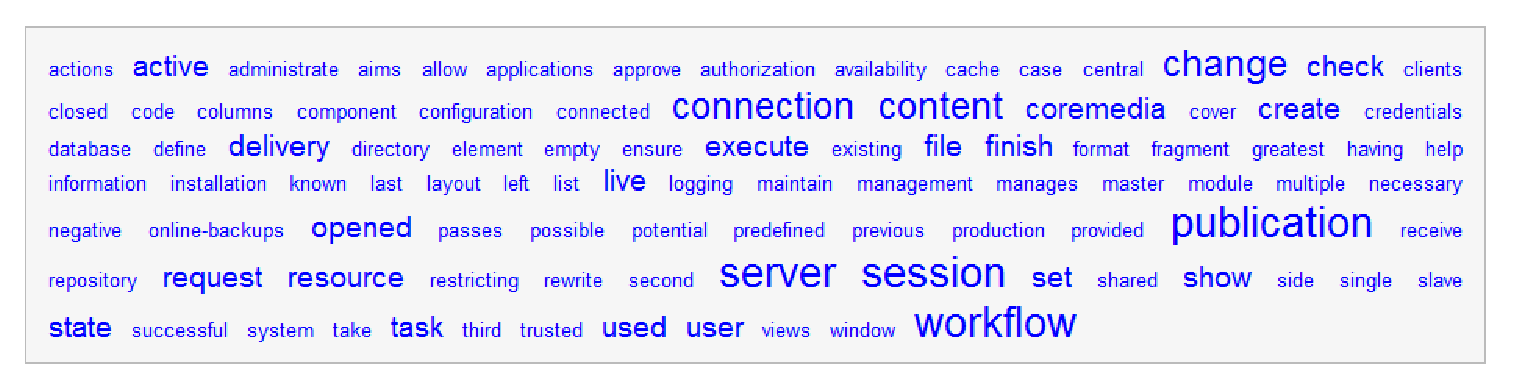
\includegraphics[width=\ScaleIfNeeded]{img/tagcloud} 
 % or [scale=0.5]
	\caption[A tag cloud.]{A tag cloud, where tags have been selected and visually weighted according to their frequency of use. \textbf{TODO:} change with a tag cloud from CM domain. }
	\label{fig:tagcloud}
\end{figure}

\section{Introduction}
Tag clouds are simple visualization interfaces. They are wide-spread as a part of Web 2.0. Several types of tag clouds exist: \\
\begin{itemize}
\item Tag clouds generated over partial lists, such as search results. The size of tags depends on the frequency of occurrence of the corresponding terms, measure for example using $tf-idf$  measure~(section~\ref{lsa:tf-idf-section}).

\item \textit{Collaborative tag clouds}, where tag frequencies (and size) are generated over all documents in the set $D$. Collaborative tag clouds present the main concepts in the collection, where the size of tags is defined by some measure, such as frequency of occurrence. 

\item \textit{ Categorical tag clouds}, where the size of tags reflects the size of corresponding category. \\
\end{itemize}

Tag clouds can be further divided into \textit{manual} and \textit{automatic}, depending on the way they are generated. Manual tags are created in social bookmarking applications by users, while automatic tag clouds are generated based on a collection of textual resources, and a frequency measure. Clouds enhance the visualization of information, contained in a collection of resources. According to Smith~\cite{tagging2008} and Peters~\cite{folksonomiesWeb2.0_2009} tagging has the following main application areas: \\
\begin{itemize}
\item \textit{Information retrieval}, e.g. in the online services Last.fm\footnote{\url{http://www.lastfm.de/}, accessed December, 2010} or Engineering village\footnote{\url{http://www.engineeringvillage.org/}, accessed December, 2010}, where tag clouds enhance \gls{IR}, and are used to retrieve resources. Here are also included tag clouds used in e-commerce services, such as Amazon~\footnote{\url{http://www.amazon.com/gp/tagging/cloud/}, accessed December, 2010}.

\item \textit{Online libraries} use tag clouds to present book content in the form of main concepts, for example in Library Thing\footnote{\url{http://www.librarything.com/}, accessed December, 2010}, or to save bookmarks to electronic books, as in  . And these are just two examples out of many more. \\

\item \textit{Social bookmarking}. Delicious\footnote{\url{http://www.delicious.com/}, accessed December, 2010} offers tagging for sharing bookmarks to online resources, and the infamous Facebook\footnote{\url{http://www.facebook.com/}, accessed December, 2010}  uses tagging for sharing photos, videos or music. \\

\item As a part of \textit{games with a purpose}, or \textit{GWAP}\footnote{\url{http://www.gwap.com/}, accessed December, 2010}, where tagging is used for improving computer programs, such as programs performing image recognition tasks, for tagging audio or image files. \\ 
\end{itemize}

As tags and tag clouds are heavily used in collaborative tagging, an example for tag cloud use is given in the context of social bookmarking software~(fig.~\ref{collaborativeTagging}). In this application users have the roles of both content creators and content consumers. As consumers, they can use tag clouds for retrieval of resources, and visualization. In fig.~\ref{collaborativeTagging}, the tag cloud contains the most commonly occurring tags in the system, and tag bookmarks contain for a given tag $t$, a list of the most recently posted URLs annotated with $t$.  \\  

% wcc graphically presented simplified
\begin{figure}
	\centering
	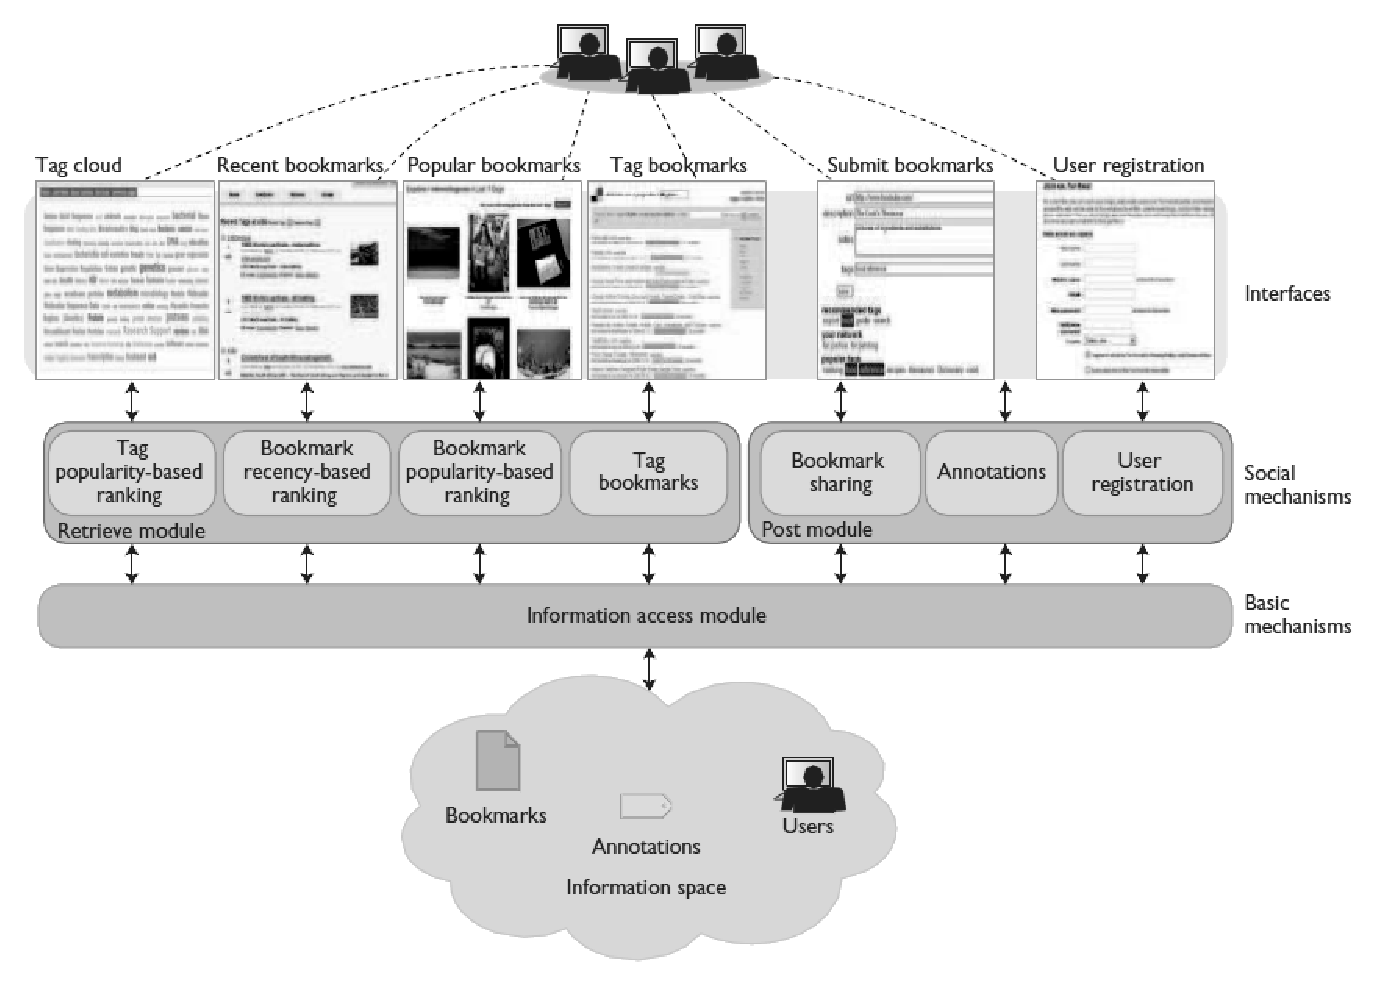
\includegraphics[scale=0.6]{img/collaborativeTagging} 
	\caption[Tag clouds in collaborative information services]
           {Tag clouds in applications for collaborative information services. Source: Heymann, Koutrika, Garcia-Molina(2007, ~\cite{tagcloud_spam2007})}
\label{collaborativeTagging}
\end{figure}

%Using tagging in social bookmarking software has definite advantages. 
The extensive amount of people involved in the process of resource tagging can overcome to some extent the flood of information, generated on a daily basis by users. With respect to social bookmarking, Clay Shirky\footnote{\url{http://shirky.com/writings/ontology_overrated.html}, accessed December, 2010}, a professor at New York University, says: \textit{"The only group that can categorize everything is everybody."}. However, social tagging has certain drawbacks. There is criticism about the quality of tagging, as it is usually done by laymen, and privacy issues arise, concerning the content tagged by users~\cite{folksonomiesWeb2.0_2009}. \\


\section{Tag clouds generation}
Tag clouds are generated from a collection of tags, and corresponding weights associated with them, which measure the "importance" or define the tag size in the cloud. The implementation usually includes a preprocessing phase, as already discussed in section~\ref{sec:lsa:doc_repres}, such as text parsing, filtering out of stop words, numbers, punctuation. As tag size is defined by frequency of occurrence, for small frequencies size is normalized to one. For larger values, a normalization is applied. In a linear normalization, the weight $t_{i}$ of a tag is mapped to a size scale of $1$ through $f$, where $t_{min}$ and $t_{max}$ are specifying the range of available weights. Thus, the displayed font size of a tag $t_{i}$ is defined by: \\
\begin{equation}
f_{i} = \lceil {\frac{f_{max} . (t_{i} - t_{min})}{(t_{max} - t_{min})} }\rceil \mbox{ for }  t_{i} > t_{min}; \mbox{ else }  f_{i} = 1
\end{equation}

where $f_{i}$ is the displayed font-size, $f_{max}$ is the maximum font-size, $t_{i}$ is the count of tag $t$, and $t_{min}$, $t_{max}$ are limits for minimum and maximum count that a term $t$ can have. \\

\textbf{TODO:} think over.

\subsection{Tag cloud layout}
The traditional tag cloud layout is alphabetical. Tag clouds provide an aggregate of tag-usage statistics. They are typically sent as in-line HTML to browsers. Since the font size of a displayed tag is usually used to show the relative importance or frequency of the tag, a typical tag cloud contains large and small text interspersed. The following kinds of layout are common: \\

\begin{itemize}
\item Sequential layout, with either a horizontal or vertical arrangement of tags, sorted
alphabetically or by some other criteria (e.g., popularity, chronology, etc.).

\item Circular layout, with the most popular tags in the center and tags with decreasing
popularities towards the borders (or vice versa).
 
\item Clustered layout, in which the distance between tags follows a certain clustering
criteria (e.g., semantic relatedness) and related tags are positioned in close
proximity [3, 6].
\end{itemize}



\section{Existing implementations}
In this work, a semantic space is constructed over a set of documents using \gls{LSA}~(Chapter \ref{sec:lsa}), and a tag cloud is used to visualize the main concepts in search results, retrieved from this space. Similar implementations of tag clouds exist, used to enhance \gls{IR} tasks. Examples of such applications are given below. \\

\textbf{Yippy}\footnote{\url{http://cloud.yippy.com/}, accessed Dezember, 2010} is a tool that visualizes topics based on search queries as a tag cloud, previously known as Clusty. Created by Vivisimo\footnote{\url{http://vivisimo.com/}, accessed Dezember, 2010}, it offers classification of search results. \\

Google\footnote{\url{http://www.google.com/}, accessed December, 2010} has developed their \textbf{Wonder wheel} search visualization tool, in order to display search results as a categorical tag cloud. The tags in Google's Wonder wheel represent categories in the set of search result documents. \\ 

\textbf{Opinion Crawl}\footnote{\url{http://www.opinioncrawl.com/}, accessed December, 2010} - web sentiment analysis application. It generates a concept cloud from daily scanned blogs, web site articles, and is developed at Semantic Engines LLC.\\

\textbf{SenseBot Search Results} is another tool from Semantic Engines LLC. It is a plugin for Mozilla Firefox browser that generates a tag cloud of the main concepts returned as search results from Google, included as a part of the SenseBot semantic search engine\footnote{\url{http://www.sensebot.net/}, accessed December, 2010}.\\

These are just a few examples of tag cloud usage presented here, as they are similar to the implementation purpose of the tag cloud developed in this work.  \\


\section{Conclusion}
In this chapter tag clouds were presented as visualization interfaces for enhancing \gls{IR} services, and discussed the use of tag clouds in the context of social bookmarking applications, and commercial retrieval systems. In the next chapter, the tag cloud implementation is given, which was developed as a part this work, and its function as a part of an \nopagebreak \gls{IR} process is explained. \\



